\section{Experiments}

We investigate how SILVR can improve an in-domain video model initially trained on a limited set of demonstrations and tasks to further solve novel robotic control tasks through self-collected experience.  We focus on two main robot settings to evaluate SILVR: the MetaWorld-v2~\citep{yu2020meta} simulated environment, and a real-world Franka Emika Panda robot arm.  We describe our experimental setup for each environment, as well as different design decisions considered.

\subsection{Experimental Setup and Evaluation}
\label{sec:experimental_setup}
\textbf{Synthetic Environment:} MetaWorld encompasses a wide selection of tasks, allowing us to thoroughly assess visual planning performance trends through SILVR for many choices of held-out novel tasks.  Furthermore, MetaWorld provides ground-truth success evaluations, enabling strictly quantitative comparisons on task performance as well as iterative improvement abilities.  For MetaWorld experiments, we first collect 25 demonstrations from 8 different tasks (denoted with an asterisk in Table~\ref{table:text_prompts}) for initial in-domain video model and inverse dynamics model training. Subsequently, we instantiate SILVR with both models on 12 unseen tasks for self-improvement. In each SILVR iteration, we collect 30 trajectories rendered from the environment via visual planning, and finetune both in-domain video model and inverse dynamics model using filtered successful data. Due to the sim-to-real gap, we disable the use of internet-scale video prior in MetaWorld by default.


\begin{table}[t]
\centering
\setlength{\tabcolsep}{4.8pt}
\scalebox{0.9}{
\begin{tabular}{@{}lccccc@{}}
\toprule
Iteration & 0               & 1               & 2               & 3               & 4                \\ \midrule
DSRL (w/ GT Filter)      & 9.4 ($\pm$1.7) & 8.3 ($\pm$1.6)  & 7.4 ($\pm$0.9)  & 7.5 ($\pm$3.4)  & 7.7 ($\pm$3.4)   \\
BCIL (w/ GT Filter)      & 5.6 ($\pm$0.6)  & 12.3 ($\pm$2.3) & 20.9 ($\pm$1.6) & 23.3 ($\pm$0.4) & 23.2 ($\pm$0.9)  \\
SILVR (w/ GT Filter)     & 14.7 ($\pm$0.6) & 27.7 ($\pm$1.9) & 33.5 ($\pm$2.2) & 43.5 ($\pm$2.6) & 44.2 ($\pm$4.5)  \\
SILVR (w/ VLM Filter)      & 17.0 ($\pm$0.6) & 24.4 ($\pm$0.9) & 28.7 ($\pm$2.8) & 34.4 ($\pm$1.4) & 38.4 ($\pm$1.3)  \\\midrule
SILVR-Distilled DP &                 &                 &                 &                 & 44.2 ($\pm$4.5) $\rightarrow$ 49.2 ($\pm$3.4) \\ \bottomrule
\end{tabular}
}
\caption{\textbf{SILVR Results on MetaWorld}. We report the average performance over 12 unseen MetaWorld tasks for SILVR and all baseline methods, each aggregated over three seeds. We also provide the performance of diffusion policy distilled from the video model from the last SILVR iteration, denoted as ``SILVR-Distilled DP". SILVR outperforms all baselines by a large margin since Iteration 1. Furthermore, SILVR-Distilled DP achieves the best overall performance.}
\label{table:silvr_baseline_results}
\end{table}

\begin{figure}[t]
    \centering
    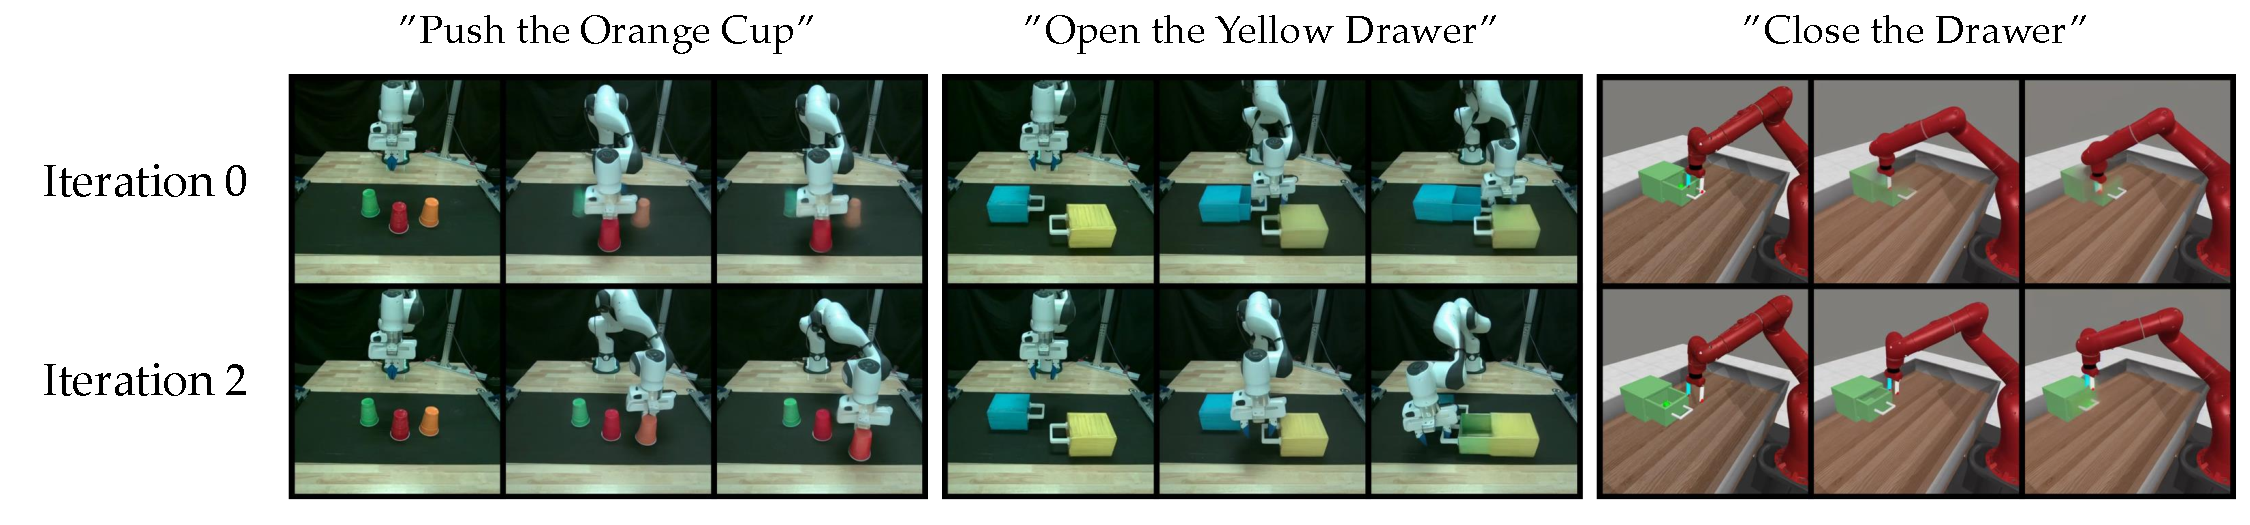
\includegraphics[width=\linewidth]{figures/full_task_visual_plan_comparison_3.pdf}
    \caption{\textbf{Qualitative results on visual plans improvement.} We illustrate visual plans for a variety of tasks and settings at Iteration 0 (top) and Iteration 2 (bottom) with random initial object locations. Although the visual plan at Iteration 0 renders blurry objects and fails to complete the specified tasks, our approach synthesizes the correct visual plan (with slight color drift) after two SILVR iterations.}
    \label{fig:franka_sail_visual_plans_comparison_all_tasks}
\end{figure}


\textbf{Real-World Environment:} Deploying SILVR on a robot arm in the real world demonstrates the practicality of the approach, as well as tests robustness to real-world confounding factors such as lighting conditions.  In one experiment, we utilize a Franka Emika Panda robot arm for the task of pushing cups specified by a user-provided text prompt.  In contrast to the MetaWorld setups, where each task of interest has its own distinct visual setting, we construct the cup experiment as a consistent scene setting of 3 differently colored cups (Figure~\ref{fig:sail_teaser}). Success is then measured in terms of whether the robot arm can accurately locate a specified color cup and push it forward.  To test generalization, conditioned on natural language, we evaluate successful planning and execution performance on unseen cup colors.  In practice, we use a set of four colors (red, green, blue, pink) for in-domain training and two novel colors for testing generalization (orange, purple).  This translates to 12 possible unique tasks formed from combinations of the seen colors, and we train our in-domain video model with 10 human-teleoperated demonstrations of each for a total of 120 training videos. Then, generalization evaluation is calculated as an average over 5 rollouts for every possible pair combination of the seen color set combined with the novel color, for a total of 30 videos. For both novel colors, we initialize SILVR using the same pretrained in-domain video model. In each SILVR iteration, we combine self-collected data with the initial demonstrations for in-domain finetuning.

In a second real-robot experiment, we utilize the Panda arm to select and open a drawer specified via a user-provided text prompt.  The scene is constructed as two distinctly colored closed drawers, where the robot is prompted with one particular color and expected to open its corresponding drawer.  We use a set of three colors (red, green, blue) for in-domain training and one novel color (yellow) for testing generalization.  With 24 possible drawer placement combinations for each ordered pair of seen colors, of which there are six, this amounts to a total of 144 human-teleoperated demonstration training videos.  Consistent with the cup pushing experiment, we use half the possible combinations for evaluation; therefore, performance is calculated as an average over 12 rollouts for every possible pairing of the novel color with a seen color, for a total of 36 self-collected trajectories per iteration.  

For both real-robot experiments, success is judged by a human for evaluation. The same success signal is also used to perform data filtering on the rollouts. We study the impact of data filtering in Section~\ref{sec:filtering_signal_silvr}, and enable adaptation with internet video priors through IPA by default.

\begin{figure}[t]
    \centering
    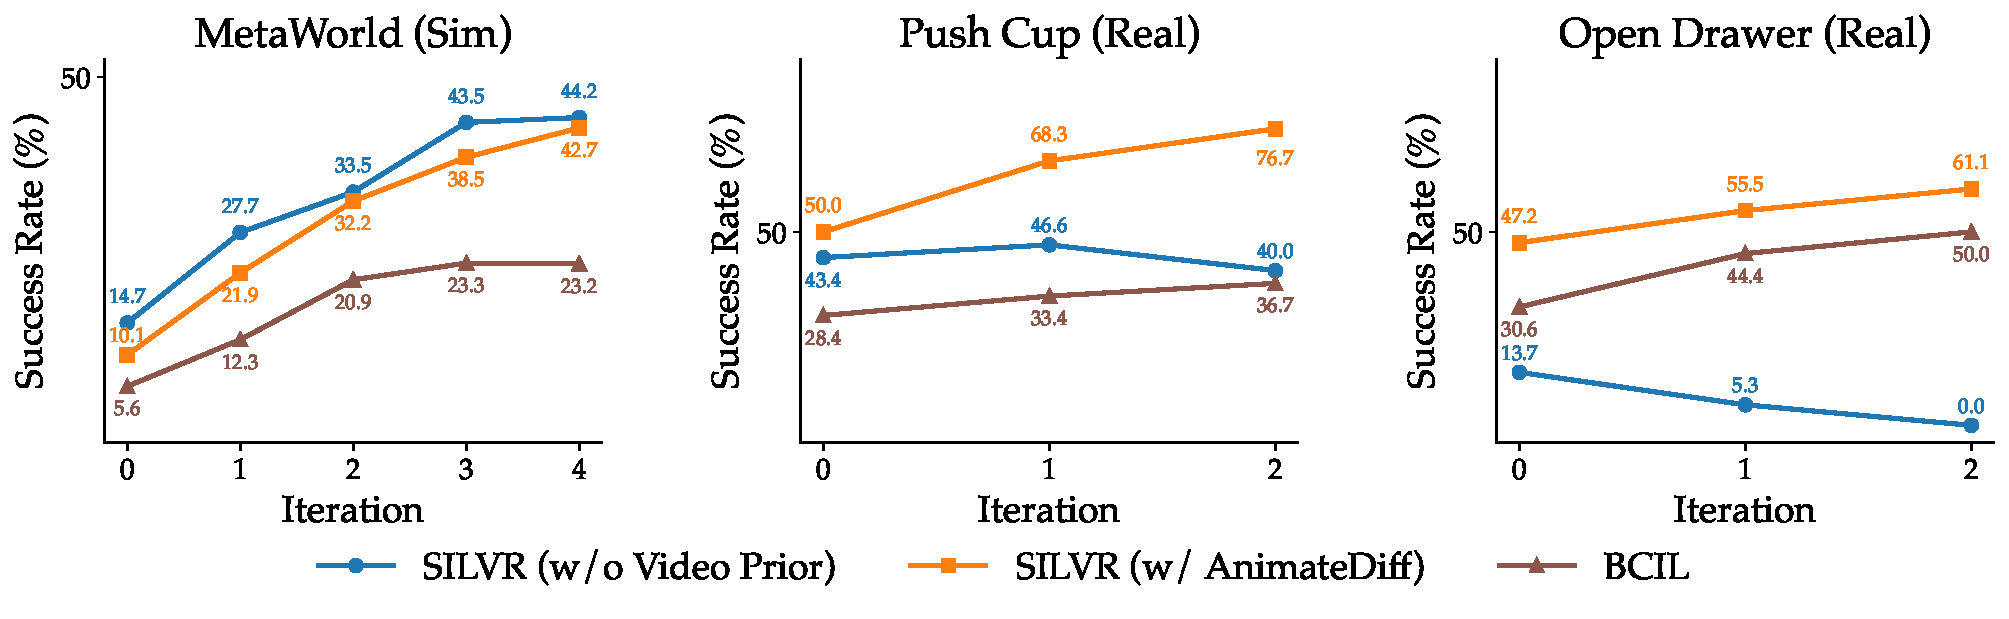
\includegraphics[width=\linewidth]{figures/sail_filter_ipa_vs_in_domain_mw_franka_combined_bc_2.pdf}
    \caption{\textbf{SILVR Results} in comparison to Behavior Cloning Improvement Loop (BCIL). We report the average performance over 12 unseen MetaWorld tasks, as well as novel pushing and drawer opening tasks for Panda arm experiments across several iterations of self-improvement (x-axis). Numbers in the graph correspond to success rate achieved (y-axis).}
    \label{fig:silvr_mw_franka_main}
\end{figure}


\textbf{Implementation Details:} We implement our in-domain video model based on AVDC~\citep{ko2024avdc}, with an added cross-attention layer to each level of the denoising U-Net to further improve text-conditioning capabilities. We train in-domain video models to predict 8 future frames conditioned on the current observation and task prompt, with a frame skip of 1 for MetaWorld and 16 for real-robot experiments. For the large-scale pretrained text-to-video model, we use AnimateDiff~\citep{guo2023animatediff} ($\sim$2B parameters), which is pretrained on WebVid-10M~\citep{bain2021webvid}.  %
Each iteration of SILVR finetunes the in-domain video model for 10,000 steps with a learning rate of 1e-6 on MetaWorld and 1e-5 on Panda Arm drawer opening tasks, and 8,000 steps with a learning rate of 2e-5 on Panda Arm pushing tasks.  We investigate two IDM implementations; one that follows prior work~\citep{luo2025solving} that implements the IDM as a MLP network that takes in the outputs of a VC-1~\citep{majumdar2023vc1} encoder model, finetuned on in-domain demonstrations.  Whereas the MLP-IDM was sufficient for real-world experiments, we found improved performance when using a Diffusion-IDM (DIDM), which is implemented as a Diffusion Policy~\citep{chi2023diffusionpolicy} with an additional goal frame provided as conditioning, for simulated settings.  Additional details on IDM design and hyperparameters are provided in Section~\ref{sec:implement_appendix}.  For MetaWorld experiments, the DIDM is iteratively finetuned on the online collected experience along with the video model.


\begin{figure}[t]
    \centering
    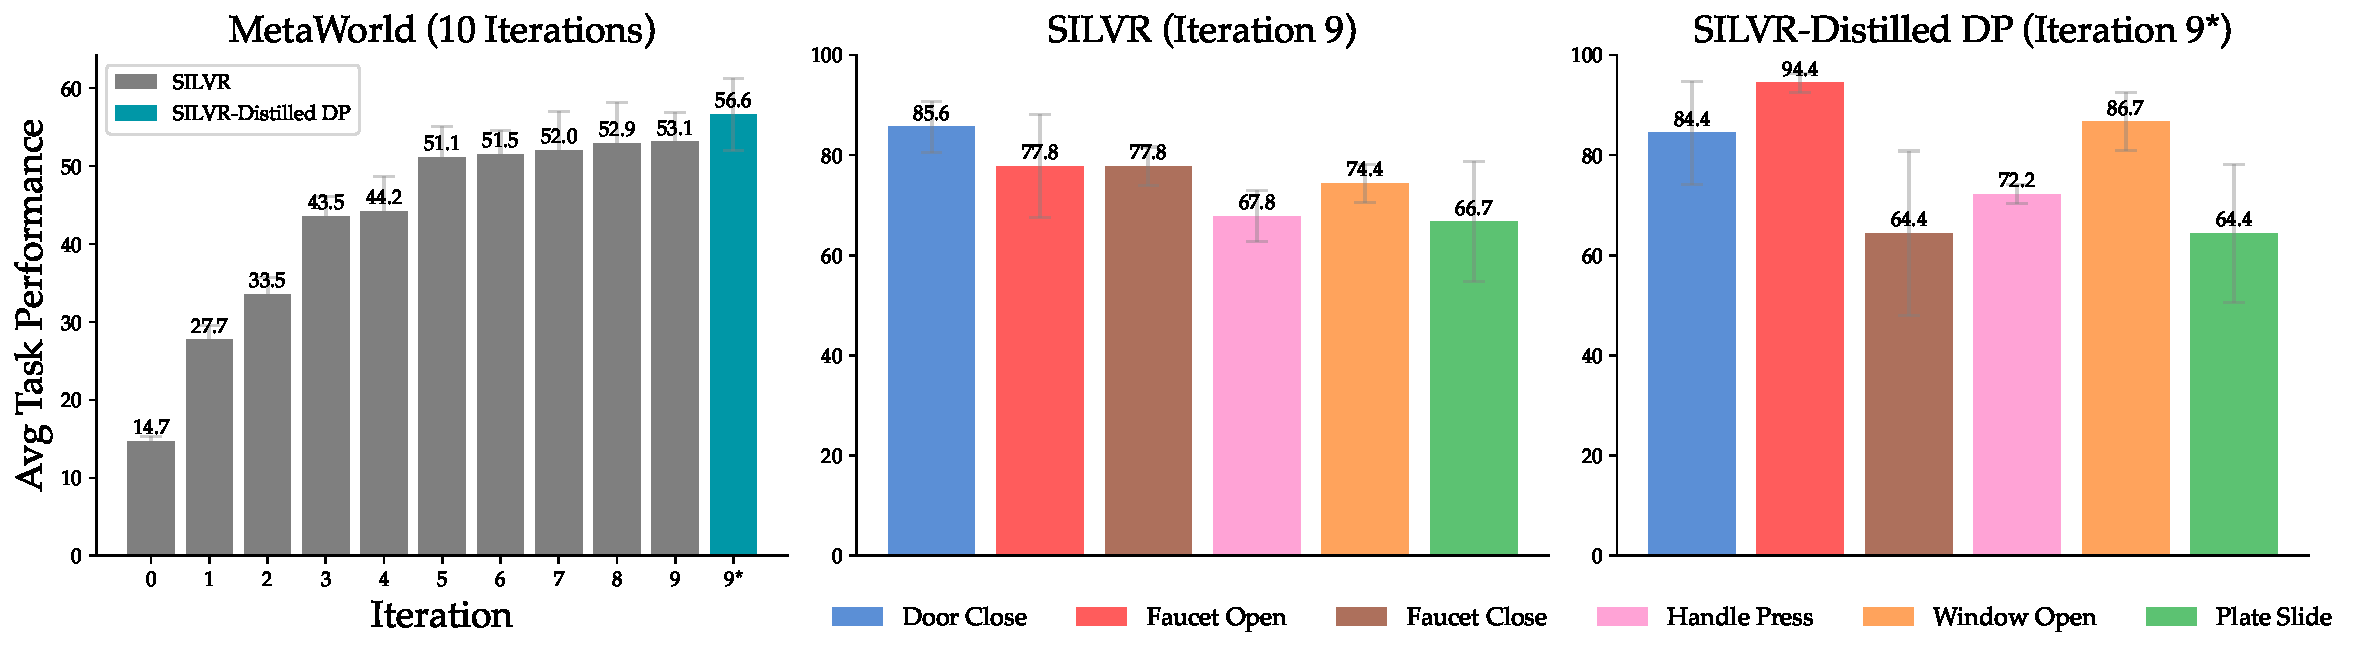
\includegraphics[width=\linewidth]{figures/mw_sail_iter10_bar_2.pdf}
    \caption{\textbf{SILVR results on MetaWorld for 10 iterations}. We report effects of training SILVR on an extended amount of iterations.  On the left plot, we show that performance continues to monotonically increase, but with diminishing improvements and effective saturation past iteration 5. On the middle and right plots we visualize a comparison between the final iteration visual planner against its distilled student BC policy from the visual planner across 6 tasks, where we observe that certain tasks actually improve after distillation.}
    \label{fig:silvr_iter10}
    \vspace{-1em}
\end{figure}

\subsection{SILVR via Filtered Finetuning}

We report incremental visual planning results for MetaWorld through five SILVR iterations, against two self-improving baseline methods built off of Diffusion Policy (DP)~\citep{chi2023diffusionpolicy}: DSRL~\citep{wagenmaker2025steering} and Behavior Cloning Improvement Loop (denoted as ``BCIL''). We initialize DSRL and BCIL with a Diffusion Policy trained on the same in-domain data as used for in-domain video model and inverse dynamics model pre-training in SILVR. We utilize the ground-truth task success signal to filter the same amount of self-collected data per iteration and finetune models with only successful trajectories.

In Table~\ref{table:silvr_baseline_results}, the performance is averaged over 12 unseen MetaWorld tasks and aggregated over 3 seeds. Despite the same initial in-domain data being shared across all methods, we observe that the visual planning approach achieves better performance than DP-based approaches at Iteration 0, laying solid foundations for subsequent improvement. Compared to DP, which learns to map observations to actions directly, visual planning decouples dynamics modeling from action prediction. We hypothesize that the separately learned environment visual dynamics is easier to transfer when solving a novel task, leading to stronger base generalization performance through visual planning. While DSRL fails to improve and BCIL quickly saturates at a low success rate after several iterations, SILVR continuously improves and consistently outperforms the baselines by a large margin, demonstrating its high sample efficiency. 














\begin{figure}[t]
  \centering
  \begin{subfigure}[b]{0.54\textwidth}
    \centering
    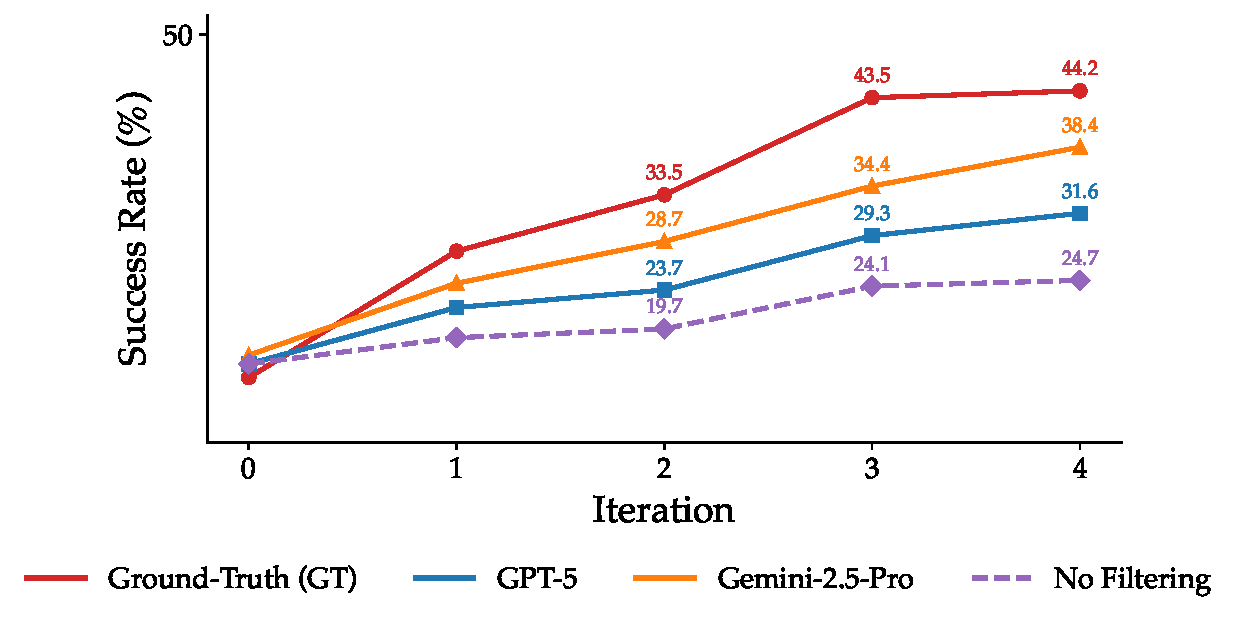
\includegraphics[width=\textwidth]{figures/mw_sail_expert_filtering_strategy_3seeds_with_vlm.pdf}
    \caption{\small MetaWorld (over 12 unseen tasks)}
    \label{fig:sail_mw_filter_ablation}
  \end{subfigure}
  \hfill
  \begin{subfigure}[b]{0.45\textwidth}
    \centering
    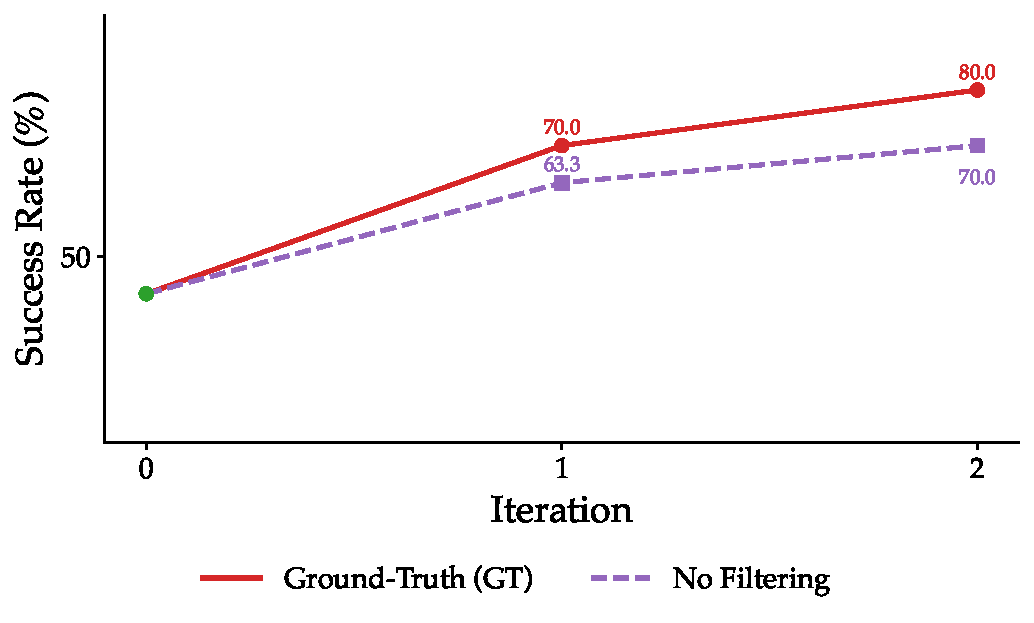
\includegraphics[width=\textwidth]{figures/franka_sail_filtering_strategy_new.pdf}
    \caption{\small Panda Arm Cup Push (Orange)}
    \label{fig:sail_franka_filter_ablation}
  \end{subfigure}

  \caption{
  \textbf{Ablations on data filtering.} We compare the effect filtering has on success rate (y-axis) across iterations of finetuning (x-axis), on both MetaWorld~(\ref{fig:sail_mw_filter_ablation}) and Panda arm~(\ref{fig:sail_franka_filter_ablation}) setups.  On MetaWorld (left plot), we further report accuracy when filtering is performed by a VLM. We observe SILVR consistently improves task even without access to ground-truth filtering signals.}
  \label{fig:main}
  \vspace{-1.5em}
\end{figure}


\vspace{-1.5em}
\subsection{SILVR with Internet-Scale Video Prior}
\label{sec:silvr_with_video_prior}
\vspace{-0.5em}
One important observation from Table~\ref{table:silvr_baseline_results} is that the generalization capability of the visual planner in solving novel tasks has a fundamental impact on self-improving dynamics. When the task of interest is exceptionally challenging or involves confounding factors, the capacity of the in-domain video model alone might not be sufficient to elicit self-improving behaviors. In the real-world experimental setup, we adapt our in-domain model with an internet-pretrained video prior, AnimateDiff, to further strengthen the zero-shot generalization and adaptability of the visual planner. In Figure~\ref{fig:franka_sail_visual_plans_comparison_all_tasks}, we qualitatively illustrate the improvements of generated visual plans after two SILVR iterations in combination with AnimateDiff. Without observing any demonstrations of the specified tasks at Iteration 0, the visual planner can synthesize plans with blurry objects where the robot arm executes the task incorrectly. On the other hand, two iterations of SILVR not only improve the clarity of the visual plans, but also demonstrate successful task completion behaviors in the same initial layout.

In the middle plot of Figure~\ref{fig:silvr_mw_franka_main}, we report the average performance of pushing cups in two unseen colors, orange and purple, aggregated over 30 rollouts per iteration. We discover that SILVR consistently improves over iterations when adapting with AnimateDiff. In the rightmost plot of Figure~\ref{fig:silvr_mw_franka_main}, we provide the SILVR results across iterations on opening a novel colored drawer, averaged over 36 rollouts per iteration, and find that SILVR bootstraps initial visual planning performance with the help of the internet video prior. However, in both real-world experiments, the visual planner struggles to improve or even continuously deteriorates without video prior. This highlights the importance of internet video prior in self-improving behavior under real-world setups with increased visual complexity and task difficulty. In simulated environments like MetaWorld, we observe that the self-improving trend occurs regardless of whether internet video priors are utilized or not, indicating that the benefits of utilizing internet priors may diminish when there is a substantial sim-to-real gap.

Consistent with our findings on MetaWorld, action-predictive behavior cloning has a lower base generalization performance and slower self-improvement trend compared with SILVR on real robots, as shown in the BCIL curves of the middle and right plots in Figure~\ref{fig:silvr_mw_franka_main}.  This highlights a key benefit of SILVR: its ability to seamlessly utilize internet-pretrained video prior for improved text-conditioned generalization and sample-efficient online improvement in real-world robotic settings.

\vspace{-0.5em}
\subsection{SILVR Saturation and Distillation}

To further understand the limits of self-improving behavior over iterations, we provide MetaWorld results for 10 SILVR iterations in Figure~\ref{fig:silvr_iter10}.  We find that SILVR saturates at Iteration 5 with marginal gains in the following iterations.  We hypothesize that this may potentially arise from discovered local minima in task-specific strategy, where similar experiences are collected until saturation.  We believe that a possible mitigation is to introduce the notion of “exploration” into the visual planning framework to avoid ``unimodal'' behavior. Such research may look into how to extract out more diverse plans from the video planner by exploiting the stochastic nature of visual generative models. We leave this investigation as promising future work.

While visual planning approaches demonstrate strong performance in task generalization, their inference speed is bottlenecked by the video generation process, which can be prohibitively expensive for downstream applications. To mitigate this, we distill the video model from the last SILVR iteration into a lightweight diffusion policy. As shown in Figure~\ref{fig:silvr_iter10}, the SILVR-distilled diffusion policy at Iteration 9 significantly outperforms the BCIL baseline and achieves the best overall performance. A slight performance increase after distillation is a trend consistently observed across iterations, such as demonstrated in Iteration 4 of Table~\ref{table:silvr_baseline_results}.  This further demonstrates that SILVR not only excels in sample-efficient task adaptation, but also supports high inference efficiency for downstream deployment via distillation.

\subsection{Impact of Data Filtering Signals on SILVR}
\label{sec:filtering_signal_silvr}
\vspace{-0.5em}
While utilizing self-collected data is a promising approach for scalable self-improvement, filtering collected experience often requires some level of human intervention, whether through manually determining successful trajectories or designing a heuristic for quality control.  We therefore investigate how different filtering techniques affect SILVR performance, or if SILVR is robust to such design decisions.  For both MetaWorld and Panda Arm settings, we compare between using a ground-truth or human-evaluated notion of success to filter what trajectories the in-domain model is finetuned on, against not using any filtering at all and utilizing all achieved trajectories irregardless of outcome. While ground-truth success signals can often be inaccessible, we investigate whether the current state-of-the-art VLMs, GPT-5 and Gemini-2.5-Pro, can provide useful task success signals and serve as a robust alternative to ground-truth signals on MetaWorld.

In Figure~\ref{fig:sail_mw_filter_ablation}, we observe that both GPT-5 and Gemini-2.5-Pro can still enable self-improving behavior across SILVR iterations when serving as a task success judge, in which Gemini achieves the best performance among all VLM filters. We also discover that without any data filtering, the improvement over each SILVR iteration appears to be marginal compared to the filtered setup. On the other hand, in Figure~\ref{fig:sail_franka_filter_ablation}, for the Panda arm, we observe that no filtering still facilitates continuous improvement over every iteration through SILVR when adapted with the internet video prior. This is an encouraging finding, as it suggests that even for settings where manual curation of experience is expensive, self-improvement can still occur.  We attribute this property to score composition~\citep{luo2025solving, yang2023probabilistic}; suboptimal demonstrations can still communicate useful information to the in-domain model, such as visuals, valid motions, and interaction dynamics of the specific deployment environment that when combined with an internet-pretrained video model can result in a final composed output plan can be both performant as well as appearing in-domain.  As such, the success rate may still improve from iteration to iteration without filtering, as the in-domain model improves its modeling of environment dynamics and visuals, even from suboptimal self-collected experience over iterations.



\begin{figure}[t]
    \centering
    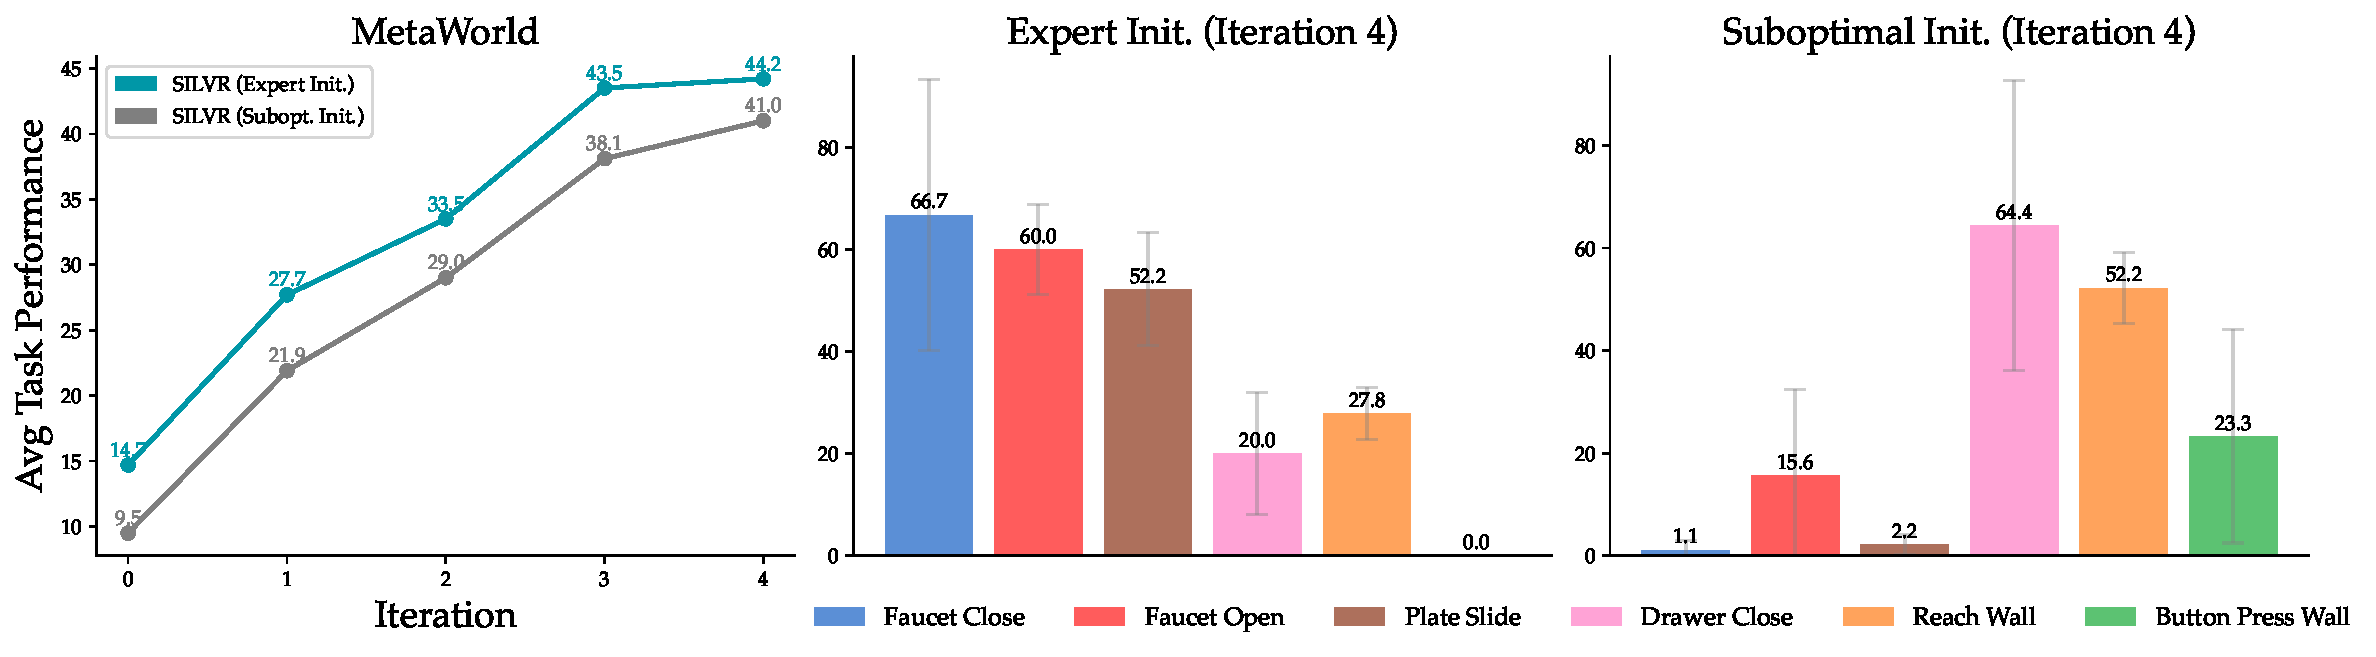
\includegraphics[width=\linewidth]{figures/mw_sail_expert_vs_suboptimal_iter5_bar.pdf}
    \vspace{-20pt}
    \caption{\textbf{Ablation studies on in-domain data quality}. On the left plot, we report SILVR performance averaged over 12 novel tasks and 3 seeds when the provided initial demonstrations of seen tasks are expert-quality or suboptimal.  We find that SILVR successfully self-improves despite suboptimal data initialization.  
    In the middle and rightmost plots, we visualize 6 tasks that have the most distinctive performance between expert and suboptimal SILVR initializations at the final iteration.}
    \label{fig:silvr_expert_vs_suboptimal}
    \vspace{-1.0em}
\end{figure}

\subsection{SILVR with Suboptimal Data}
\label{sec:suboptimal_sail}
\vspace{-0.5em}
Visual planners are usually trained explicitly on expert in-domain demonstrations, which communicate not only environment-specific visual characteristics, physics, and interaction dynamics to the generative model during optimization, but also a notion of success and optimal behavior.  However, for arbitrary environments, such expert-quality in-domain data can be expensive to collect and curate at scale.  On the other hand, suboptimal demonstration data, such as utilizing random actions during the collection procedure, may generally be cheaper to gather; however, training on a large dataset of low-quality data may not result in a performant visual planning model capable of generating plans worth following.  A natural question is how robust SILVR is to initialization data, or whether a performant video planner can still be created when only suboptimal demonstrations are available.

In our setting, we construct suboptimal data as simulated trajectories where 70\% of the time a random action is selected and 30\% an expert action is utilized.  As a consequence of this interaction procedure, the resulting trajectories are unable to successfully solve complex tasks.  
In MetaWorld we find that SILVR still demonstrates continuously improving behavior when initialized with suboptimal data, as shown in the leftmost plot of Figure~\ref{fig:silvr_expert_vs_suboptimal}, highlighting the robustness of SILVR to initial data quality. Additionally, we select 6 tasks whose performance differs most between the expert and suboptimal setup, and report their performance on Iteration 4 in the middle and rightmost plots of Figure~\ref{fig:silvr_expert_vs_suboptimal}. We find that Faucet Open, Faucet Close and Plate Slide benefit most from initialization with expert demonstrations, indicating that the skills acquired from seen tasks can be essentially useful when solving these novel tasks. Meanwhile, Drawer Close, Reach Wall, Button Press Wall can benefit more from random exploration than expert actions from specific seen tasks, leading to stronger performance when the in-domain model is initially trained on suboptimal demonstrations.
